\subsection{Anadolu Selçuklular Galerisi}
\indent\indent Müzenin bu kısmında Anadolu Selçuklu dönemine ait halı ve kilimleri geniş yer kaplıyor. 13.yüzyıldan kalma olan olan eserler, Anadolu'nun en eski halı ve kilim örneklerini oluşturmaktadır. Salonun ortasındaki vitrinde ise Anadolu Selçuklu döneminden kalma maşrapalar, vazolar, mataralar ve sürahiler bulunmaktadır. Bunlarla birlikte, yine bu döneme ait savaşçı ve grifon figürlü mermer kabartmalar bulunmaktadır.\newline
\begin{figure}[H]
    \centering
    \subfigure[Grifon Kabartması]{
        \includegraphics[height=0.3\textheight,width=0.3\textheight,keepaspectratio=false]{assets/grifon_as.jpg}
    }
    \hspace{10pt}
    \subfigure[Savaşçı Kabartması]{
        \includegraphics[height=0.3\textheight,width=0.3\textheight,keepaspectratio=false]{assets/savasci_as.jpg}
    }
    \caption{Anadolu Selçuklu Dönemi Mermer Kabartmalar}
\end{figure}
\indent Buradaki ahşap eserler arasında Karamanoğlu İbrahim Bey İmareti'nin kapısı da bulunmakta. Karamanoğlu Beyi II.İbrahim Bey tarafından yaptırılan imaretin vakfiyesi Haziran 1432, kitabesi ise Eylül 1432 tarihlidir. Bu kapı ceviz ağacından yapılmıştır. Sağ kanat üzerinde \textit{"Karamanlı neccâr İlyas oğlu Hacı Ömer'in işidir"} yazılıdır. Sol kanattaki benzer yazıdan ise sadece \textit{"neccâr"} kısmı okunmaktadır. Kapıda dikkat çeken unsur ise sol kanattaki ahşap işçiliğinin sağ kanada oranla daha göz alıcı olmasıdır. Yine aynı imarete ait pencere kanatları da hemen kapının sol tarafında bulunmaktadır. Pencere kanadının sol kanadı da ceviz ağacından yapılmıştır. Bu kapı ve pencere kanatlarındaki ahşap işçilikleri Anadolu Selçuklu ve beylikler döneminin en nadide örneklerinden biridir.\cite{dia_6}
\begin{figure}[H]
    \centering
    \subfigure[Kapı]{
        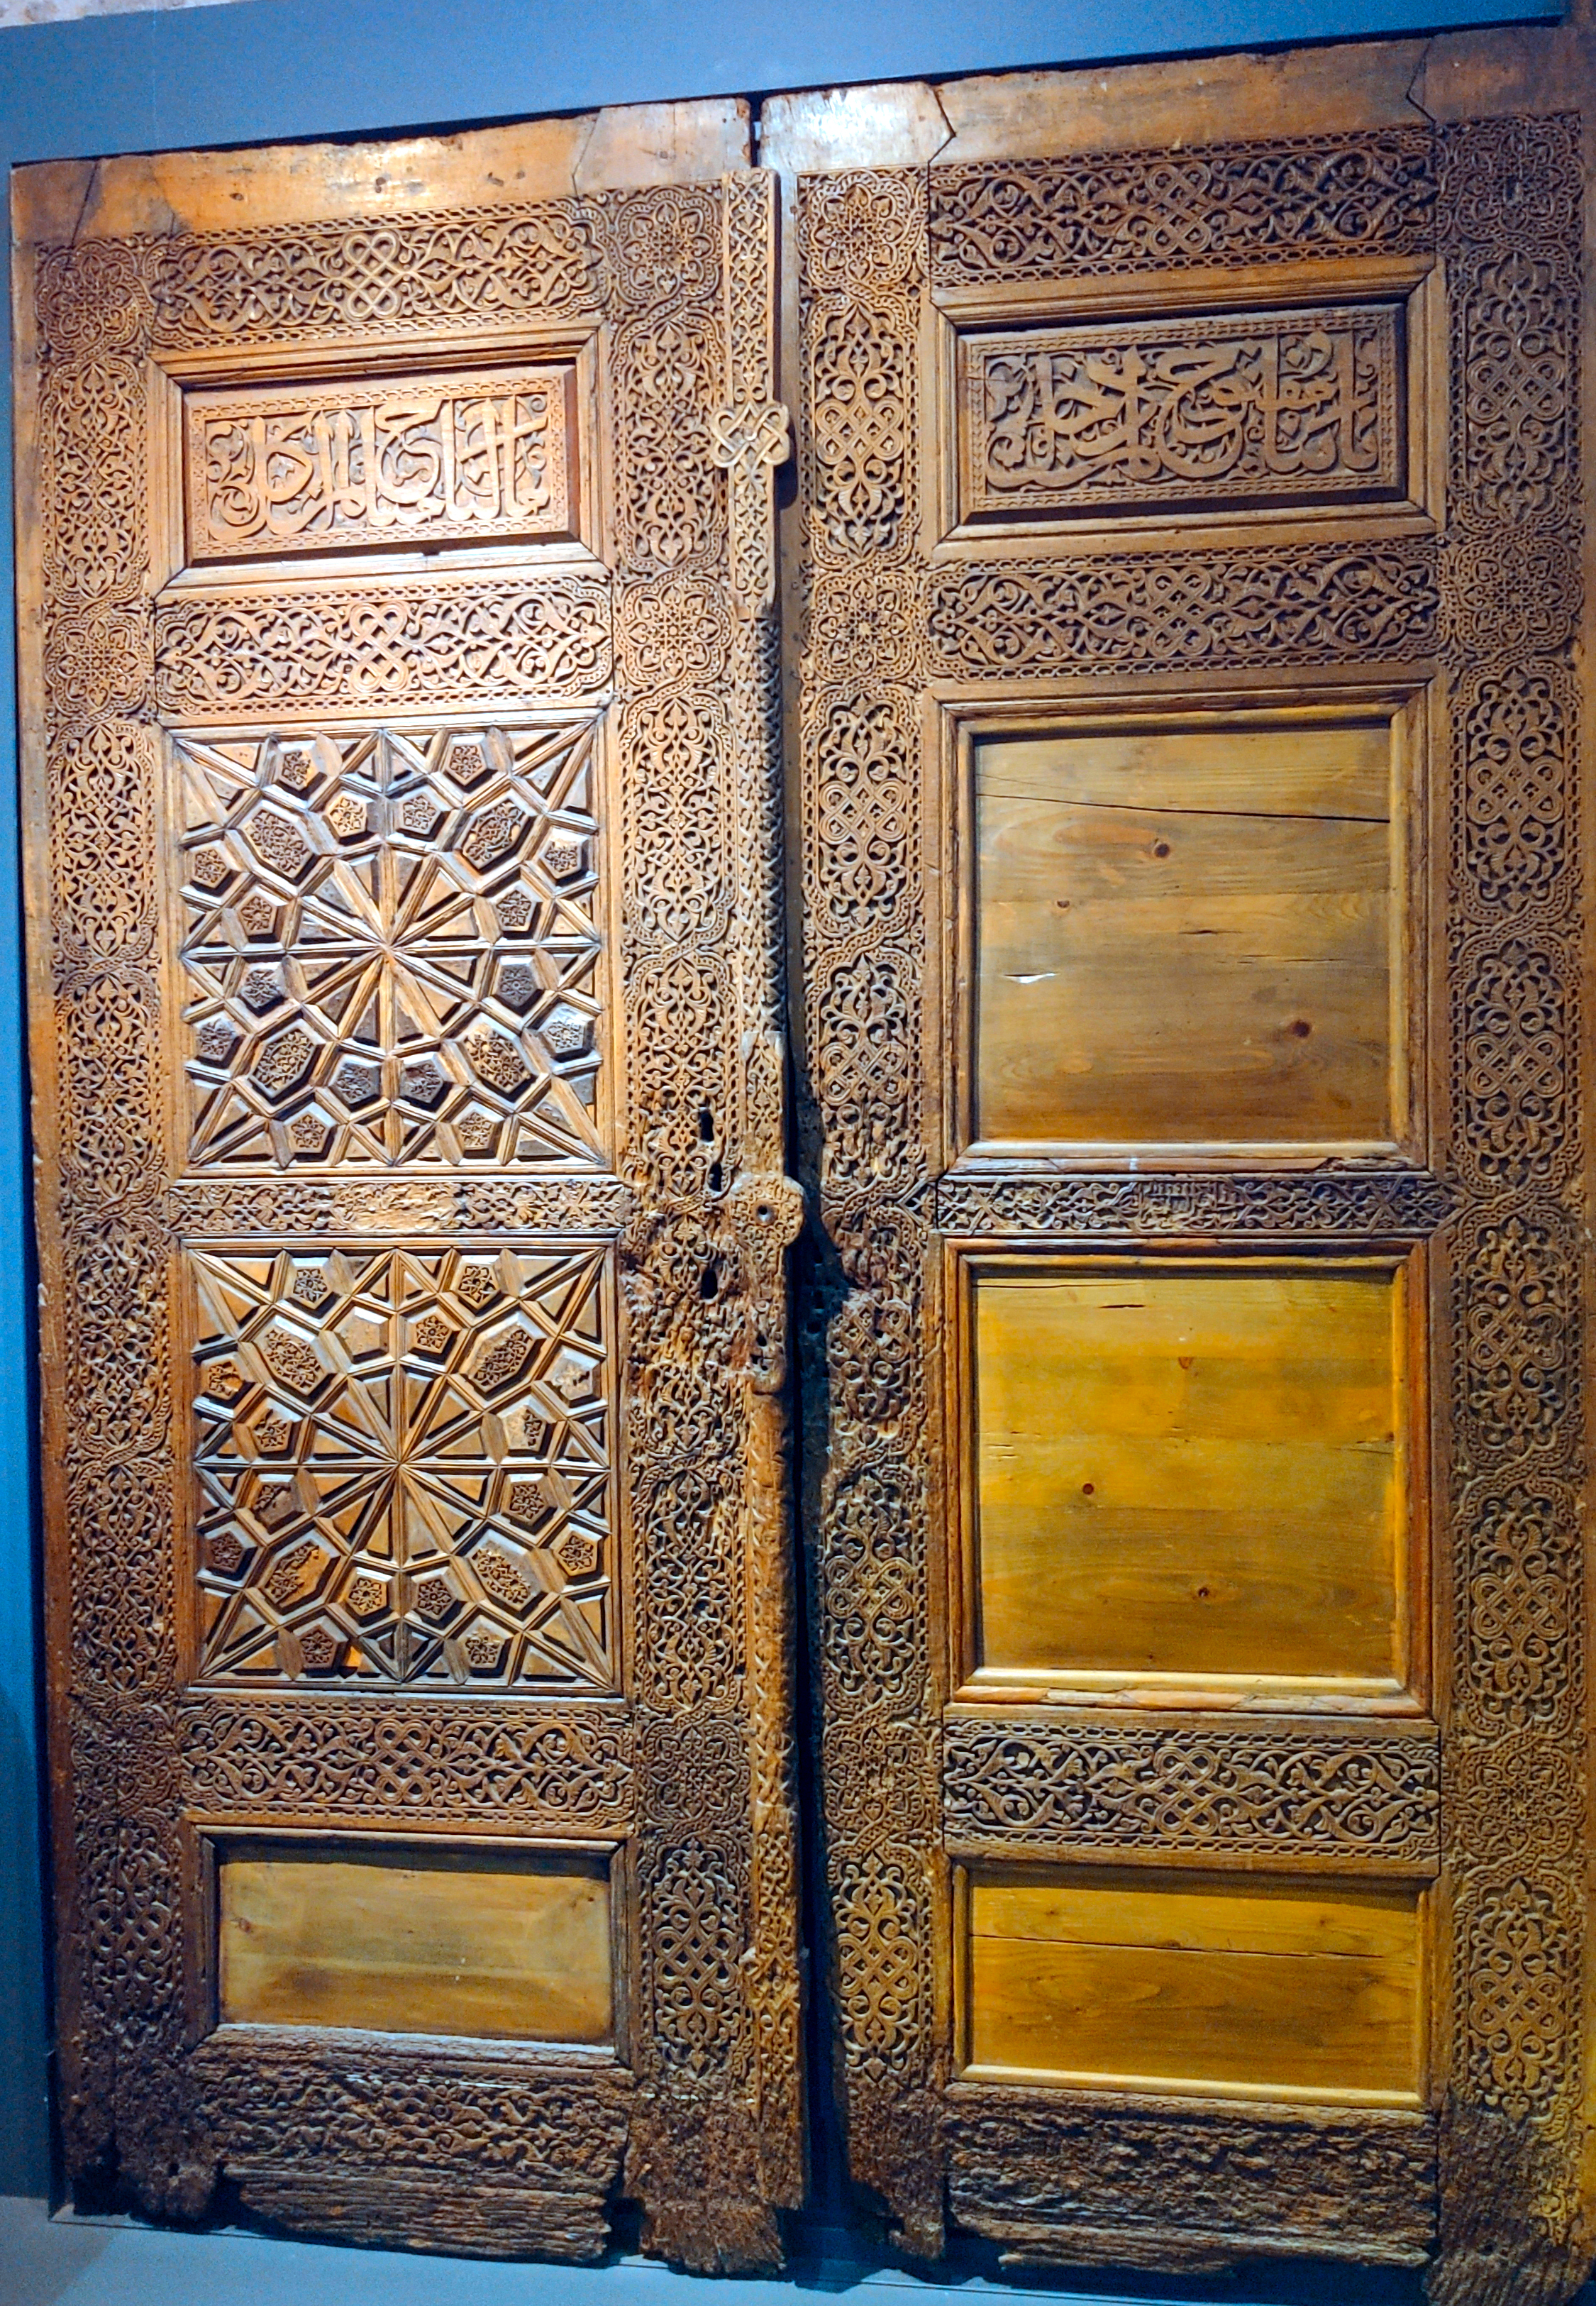
\includegraphics[height=0.4\textheight]{assets/ahsap_kapi_karaman_ibrahim.jpg}
    }
    \hspace{10pt}
    \subfigure[Pencere]{
        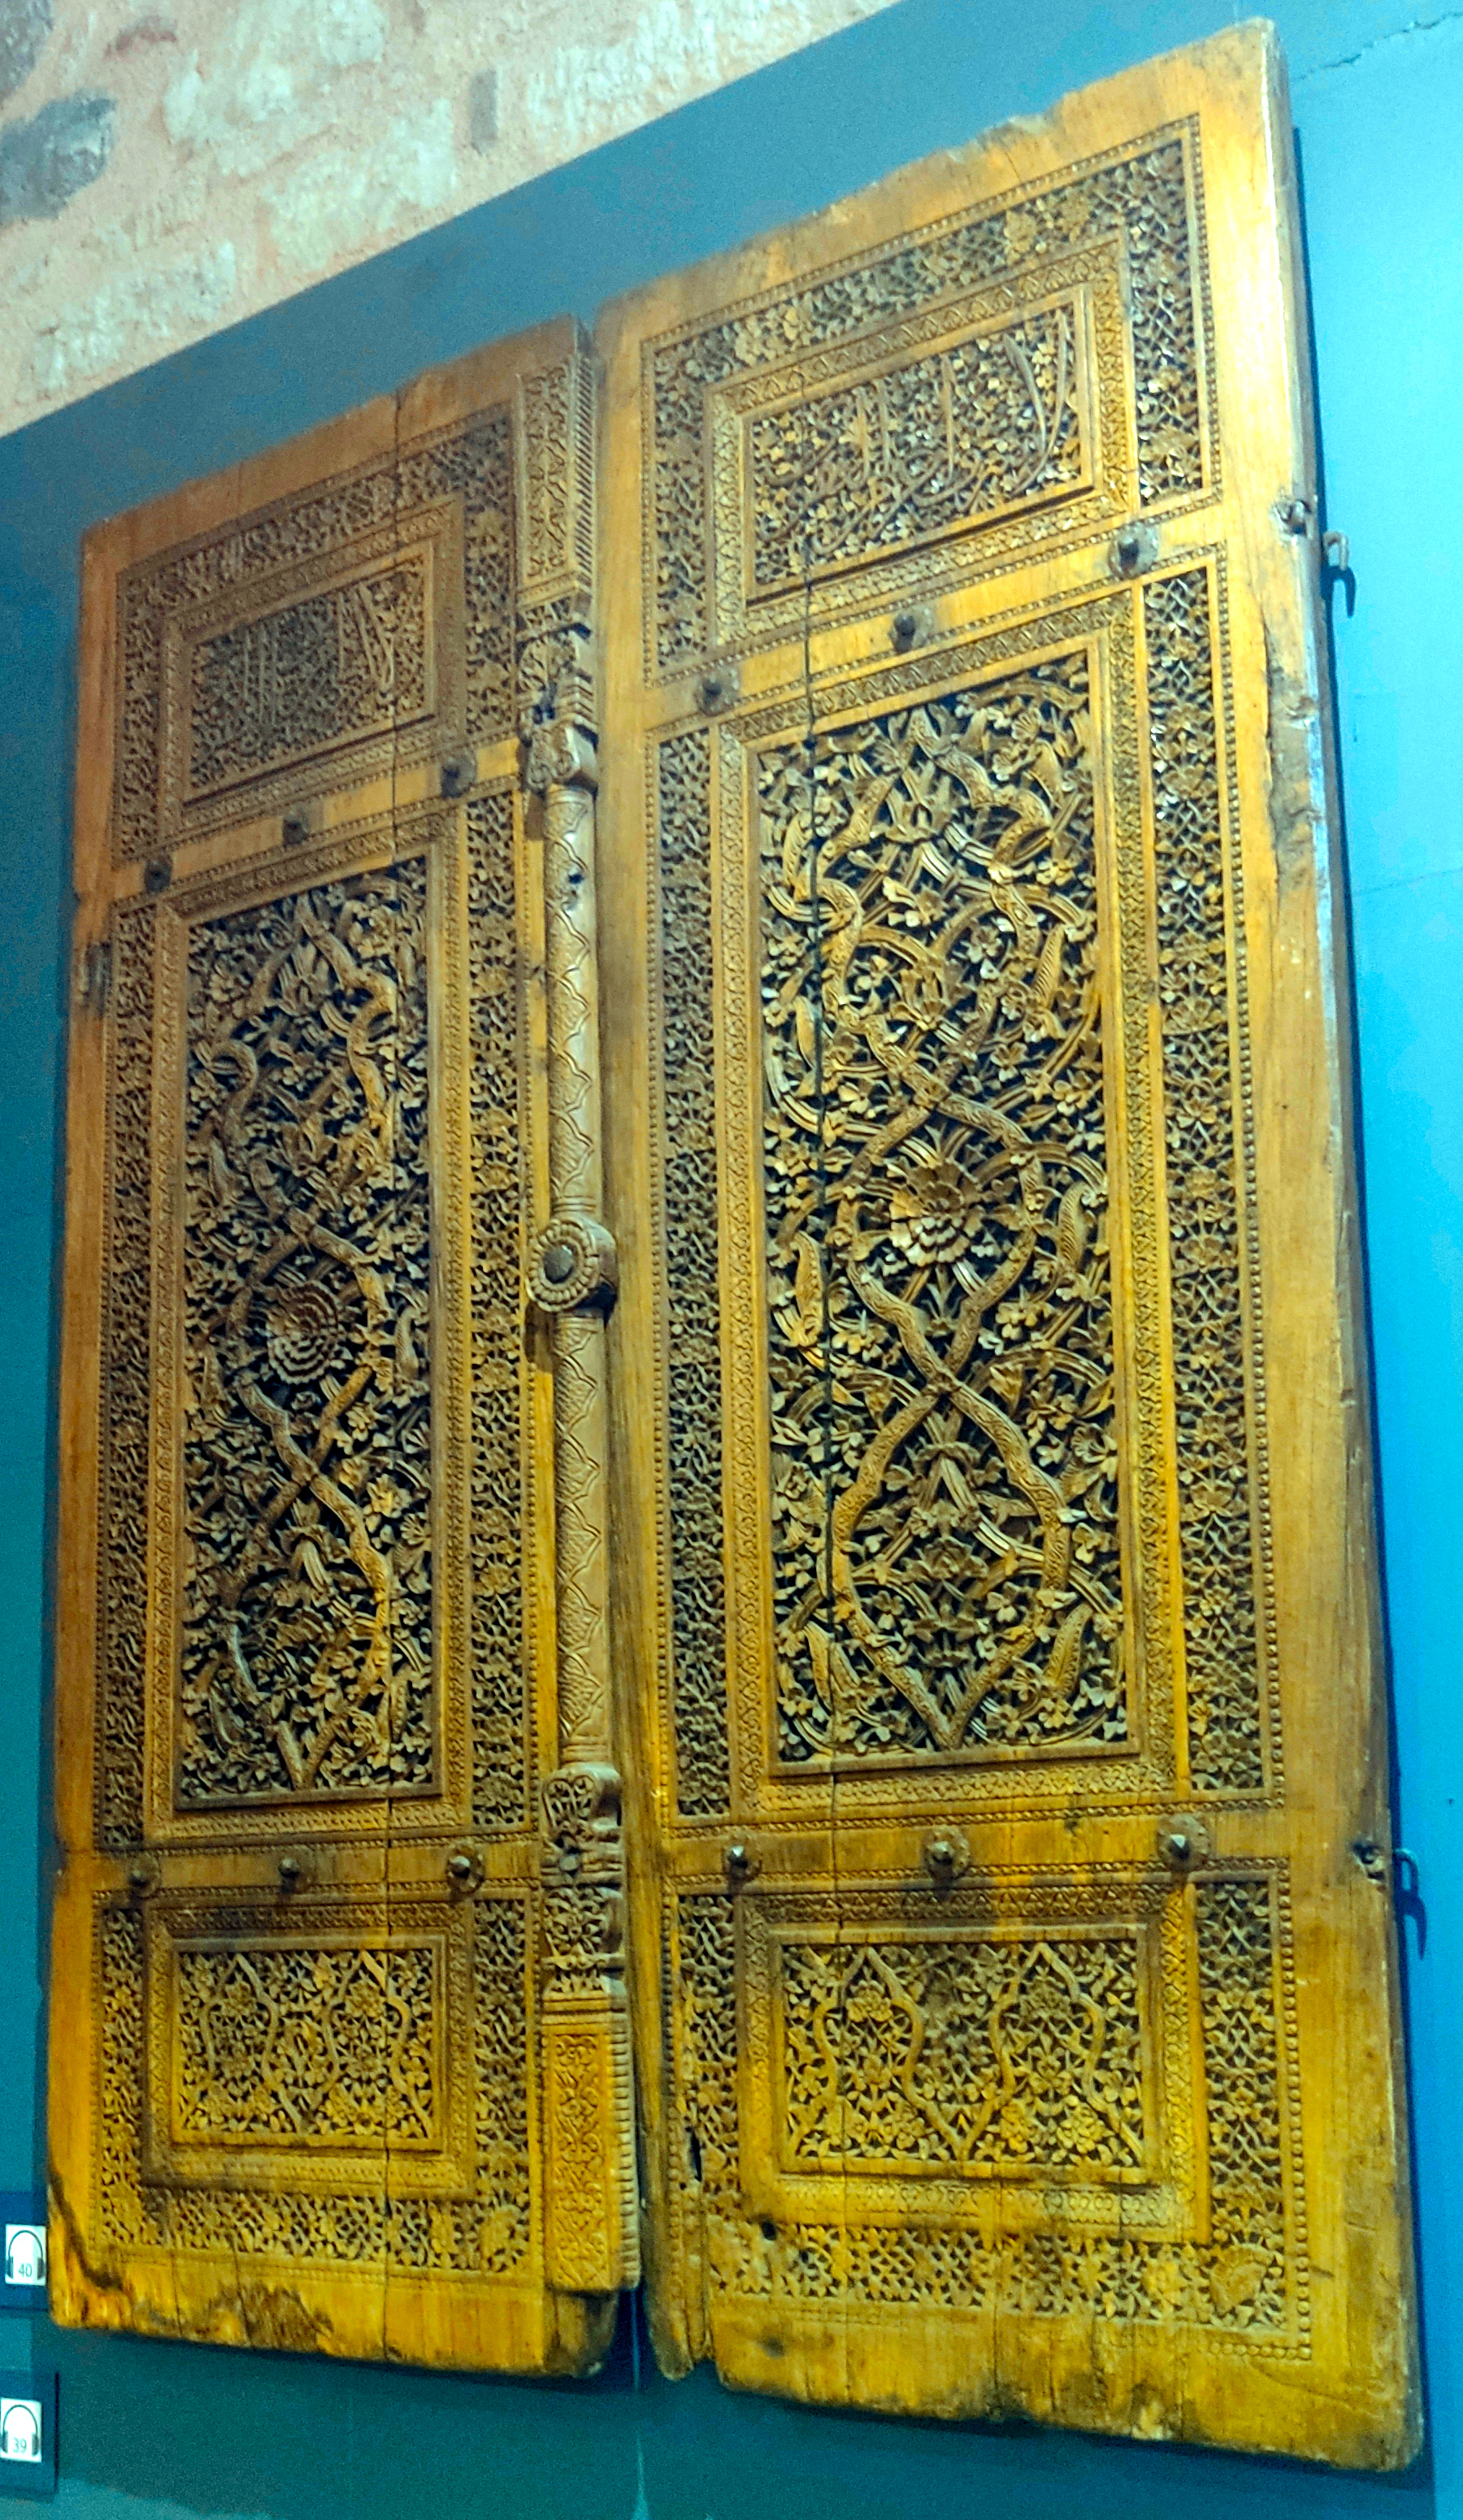
\includegraphics[height=0.4\textheight]{assets/karaman_ibrahim_window.jpg}
    }
    \caption{Karamanoğlu İbrahim Bey İmareti'nin Kapı ve Penceresi}
\end{figure}